\section{Introduction}

Parkinson's disease (PD) is a common motor neurodegenerative disorder, characterized in part by the progressive loss of pigmented dopaminergic neurons from the \textit{Substantia Nigra pars compacta}. The main neuropathological hallmark of PD is the progressive accumulation of $\alpha$-synuclein in fibrillar aggregates named Lewy Bodies (in the soma) or Lewy Neurites (in neurites) \cite{Dehay_2015}. Interestingly, Lewy pathology follows a predictable pattern of progression in the brain suggesting that $\alpha$-synuclein can propagate from neurons to neurons \cite{Braak_2003}. Such observation, common to many neurodegenerative diseases \cite{Jucker_2018}, prompted initiatives to model and predict pathology progression in the brain of patients with neurodegenerative disorders.\\
\\
In 2012, Raj and colleagues developed a Network Diffusion Model (NDM) to predict atrophy progression in dementia \cite{Raj_2012}. For this purpose, they compared Magnetic Resonance Imaging acquisitions from healthy young subjects, healthy old subjects, and old patients suffering from either Frontotemporal Dementia or Alzheimer's Disease. Their study suggested that patterns of atrophy within the dementia spectrum could be explained by transmission of the disease along neuronal pathways. Using their model, they demonstrated a path for predicting future atrophy in individuals starting from baseline. The NDM model was later applied to other diseases using various kinds of data. In 2017, Mezias and Raj showed in a mouse model that the spread of amyloid-$\beta$ pathology, involded in Alzheimer's disease, was driven by spatial proximity but not network connectivity \cite{Mezias_2017_abeta}. At the opposite, progression of tau pathology, also involved in Alzheimer's disease and other tauopathies, was better recapitulated by connectivity \cite{Mezias_2017_tau}. In 2019, Henderson and colleagues reported that progression of $\alpha$-synuclein pathology, similary to tau pathology, is largely predicted by anatomical connectivity between brain structures \cite{Henderson_2019}.\\
\\
We here replicated the  core of the NDM applied to $\alpha$-synuclein spread in mice as implemented by Henderson and colleagues \cite{Henderson_2019}. R scripts, connectivity matrix and experimental datasets were made fully accessible by the authors on GitHub allowing an easy process. We were able to reproduce qualitatively and quantitatively the main results of the publication. The aim of the present replication is not to fully replicate the entire paper but to focus on the core model and immediate results (shown in Figures 4 and 5 in the original paper).\\
\\

\section{Background}
\subsection{Graph Theory and brain connectivity}
Henderson et al. combined quantitative pathology mapping in the mouse brain with network modeling to understand the spatiotemporal pattern of spread of  $\alpha$-synuclein pathology \cite{Henderson_2019}. Graph theory is a branch of mathematics applicable to Neuroscience. The brain is a complex system that can be modeled as a network or graph. When applied properly, Graph theory can offer important insights into different aspects of brain networks such as architecture, evolution, development, or clinical disorder \cite{Sporns_2018}.\\
\\
Networks are defined as a collection of elements (or nodes) and their pairwise links (or edges) that can be summarized in the form of a connectivity matrix (named adjacency matrix). Depending on the type of graph, edges can have binary values (present: 1 - absent: 0) or actual weights reflecting connection strength. A graph is called undirected when an edge $e$ reciprocally connects nodes $V_{a}$ and $V_{b}$. Conversely, a graph is named directed when the edge $e$ is projecting from $V_{a}$ to $V_{b}$ but not from $V_{b}$ to $V_{a}$.\\
\\
Thanks to the initiative from the Allen Institute for Brain Science's Mouse Connectivity Atlas (MCA), the mouse brain mesoscale connectome is now freely accessible for the neuroscience community \cite{Oh_2014}. In a matrix, connectivity is represented as "outgoing" along  rows and "incoming" along  columns. From the adjacency matrix, the in-degree and out-degree distributions can be computed as respectively the sum of all entries in the corresponding row and the sum of all entries in the corresponding column and are represented in diagonal matrices.\\
\\
The Laplacian graph is a matrix used to explore the properties of a network. It is computed using the adjacency matrix and either the in-degree or out-degree graph depending on the applications.

\subsection{Model description}
The model used by Henderson et al. requires the mouse brain connectome (discussed in the previous section) and whole brain $\alpha$-synuclein pathology quantification.\\
\\
The experimental model of $\alpha$-synuclein pathology propagation used in the study is the now classical $\alpha$-synuclein pre-formed fibrils (PFFs -  5$\mu$g) unilateral injection in the dorsal striatum of non-transgenic mice (NTG) \cite{Luk_2012, Henderson_2019}. Following inoculation, NTG mice were terminated at 3, 6, or 9 months post-injection (MPI). Brain pathology was assessed using traditional immunohistochemical methods to detect $\alpha$-synuclein phosphorylated on Serine129 (p-$\alpha$-syn). Quantification (as percent of region occupied by immunostaining) was performed on both brain hemispheres (ipsilaterally and contralaterally to the injection point) in 58 different regions. Thus, the p-$\alpha$-syn dataset provided by the authors on their repository is an CSV sheet with values for 5 mice per group and timepoint for all 116 brain regions.\\
\\
Using the dataset from \cite{Oh_2014} for synaptic connection, the authors generated a directed and weighed connectivity graph $G={V,E}$ whose nodes $V$ are $N$ cortical and subcortical grey matter regions and whose edges $e_{ij} \in E$ represent an axonal projection from $V_{i}$ to $V_{j}$. They then defined the weighed adjacency matrix of $G$ as $A = [A_{ij}]$ generating a final parcellation of 116 regions.\\
\\
The magnitude of the observed p-$\alpha$-syn staining of all $N$ nodes at a time $t$ is the vector $x_{t}$. The predicted regional p-$\alpha$-syn $\widehat{x_{t}}$ is a function of the adjacency matrix $A$ and a seed region $seed$ ($\in E$)  and is computed as shown in (1):

\begin{equation}
    \widehat{x_{t}}=e^{-cLt} x_{o}
\end{equation}

Where:
\begin{itemize}
\item $c$ is a constant designed to achieve an optimal match with the data as the empirical diffusion constant for the pathology is \textit{a priori} unknown.
\item $t$ stands for the timepoint of the prediction. 
\item $L$ is the out-degree Laplacian matrix computed as shown in (2):

  \begin{equation}
    \begin{cases}
      -A_{ij} & \text{for $i \neq j$} \\
      \sum_{j=1}^N A_{ij} & \text{for $i=j$} \\
  \end{cases}
\end{equation}
\item  $x_{0}$ is the seed vector computed as shown in (3):
  
  \begin{equation}
    x_{0}
    \begin{cases}
        0 & \text{for $i \neq seed$} \\
        1 & \text{for $i = seed$} \\
    \end{cases}
  \end{equation}
\end{itemize}
   
\section{Material and Methods}
Henderson et al. coded their model using R and MATLAB. Codes and dataset were made fully accessible on \href{https://github.com/ejcorn/connectome_diffusion}{GitHub} by the authors. In order to only rely on opensource and free tools, we decided to reproduce the model in Python 3. We looked for operating systems intercompability and ran our code successfully on both Microsoft Windows 10 and MacOS 11.2.3. \textbf{Table 1} lists the required packages and their versions. Our code (and the associated datasets) is fully accessible in a GitHub repository \url{https://github.com/MathieuBo/PathoSpreading}.

\begin{table}[ht]
\begin{center}
\begin{tabular}{ |c|c| } 
 \hline
 \textbf{Package} & \textbf{Version} \\
 \hline
 NumPy & 1.17.0 \\
 Pandas & 1.1.5 \\ 
 Seaborn & 0.11.1 \\
 Matplotlib & 3.3.2 \\
 SciPy & 1.5.2 \\
 Statsmodels & 0.12.1\\
 tqdm & 4.7.2 \\
 \hline
\end{tabular}
\caption{\textbf{Description of required packages}}
\end{center}
\end{table}

\section{Results}
\subsection{Network model of pathological $\alpha$-synuclein spread}
The model comprises a single free parameter $c$, the seed's diffusivity coefficient, that is used to scale the model to experimental results. The model is initiated by creating the seed vector $x_{0}$ for the inoculated region: here the caudoputamen (CPu). Then, the model iterates over possible the values of $c \in [0, 10]$. We selected the value of $c$ that maximizes model fit, defined as the Pearson's correlation $r$ between $\log_{10}x_{t}$ and $\log_{10}\widehat{x_{t}}$ averaged over all timepoints. \textbf{Table 2} summarizes the results including selected $c$ value and correlation results. Correlation results for each timepoints are also plotted in \textbf{Figure 1A-C} (to be compared with Figure4a from the original article). Overall, we obtained a perfect replication, both quantitatively and qualitatively, of the original published results.\\

\begin{table}[ht]
  \begin{center}
    \centering
    
    \begin{tabular}{|l|c|c|} % <-- Alignments: 1st column left, 2nd middle and 3rd middle, with vertical lines in between
      \hline
      
      &\textbf{Henderson et al.} & \textbf{Replication} \hspace{1cm}\\

      \hline
      Best  $c$  & $1.625$ & $1.625$ \\
      MPI 1 & &\\
            \hspace{1cm} Pearson's $r$ & $0.559$ & $0.559$\\
            \hspace{1cm} $p$-value & $8.085e^{-9}$ & $8.085e^{-9}$ \\ 
      MPI 3& &\\
            \hspace{1cm} Pearson's $r$ & $0.696$ & $0.696$ \\
            \hspace{1cm} $p$-value & $3.451e^{-17}$ &  $3.451e^{-17}$ \\ 
       
      MPI6& &\\
            \hspace{1cm} Pearson's $r$ & $0.648$ & $0.648$ \\
            \hspace{1cm} $p$-value & $2.638e^{-14}$& $2.638e^{-14}$ \\ 
      \hline
      
    \end{tabular}
    \caption{\textbf{Data correspondence between the reproduced results and the original article}. The results have been rounded up to the third decimal. $P$-values for Pearson's correlation tests were corrected for multiple comparisons using Bonferroni's method. MPI: month(s) post injection.}
  \end{center}
\end{table}

\\
Then, we performed some control experiments on the model to assess its robustness. First, as in the original article, we randomly seeded the diffusion model in all brain regions and calculated the value $c$. The 'true' seeded region (CPu) was among the best fits (97th percentile), at each timepoint (\textbf{Figure 1D}). Then, we implemented 2 additional controls: we randomly shuffled (over 150 iterations) the connectivity matrix (\textbf{Figure 1E}) and the p-$\alpha$-syn matrix (\textbf{Figure 1F}), as in \cite{Pandya_2017}. For each control experiment, we plotted the corresponding value of $r$. One can appreciate the profound performance loss in the different control experiments. Our results confirm that the spatiotemporal spread of pathological $\alpha$-synuclein is driven by connectivity.

\begin{figure}[!h]
  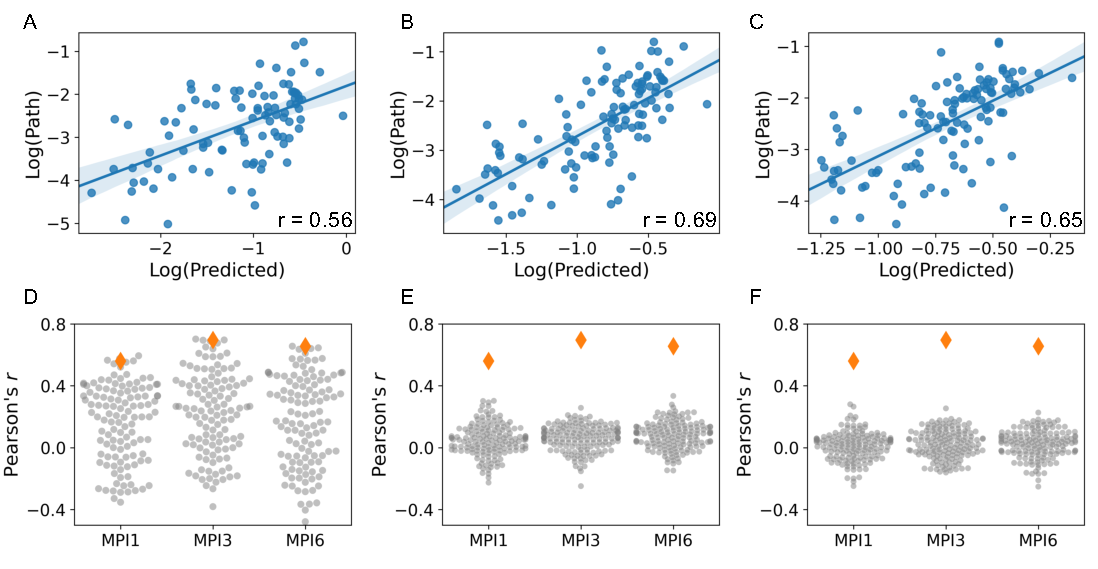
\includegraphics[width = \linewidth]{Figures/Fig1.pdf}
  
    \caption{
      \textbf{Network diffusion model based on anatomical connectivity explains pathological $\alpha$-synuclein spread.}
       (\textbf{A-C}) Scatterplots of $\log_{10}$(predicted) p-$\alpha$-syn surface versus experimentally-measured $\log_{10}$(p-$\alpha$-syn surface) values at 1 month (\textbf{A}), 3 months (\textbf{B}), and 6 months (\textbf{C}). The blue lines are the linear correlations between experimental and predicted values (shaded areas: 95\% confidence interval). Values at the bottom right of each panel are the Pearson's correlation coefficient $r$ between experiments and model's predictions.
      (\textbf{D-F}) Experimental controls: random seeding in other brain regions (\textbf{D}); shuffle of connectivity matrix (\textbf{E}); and shuffle of p-$\alpha$-syn matrix (\textbf{F}). For each control experiment, the orange marker represents the actual model fit. MPI: month(s) post injection. Path: experimentally-measured p-$\alpha$-syn surface.}
  
\end{figure}
    
\subsection{Differential regional vulnerability is correlated with $\alpha$-synuclein expression}

Intrinsic regional vulnerability is hypothesized to be a critical factor in the development of brain pathology related to $\alpha$-synuclein or other pathogenic proteins \cite{Fu_2018}. Henderson et al. thought to investigate that aspect using the connectivity-based model. To do so, they used the difference between prediction and experiment (i.e. the residues of the linear regression) as a measure of relative vulnerability. Regions with higher p-$\alpha$-syn staining than predicted were defined as vulnerable while the ones with lower values than predicted were considered resilient (\textbf{Figure 2A}). We here present an example at 6 months post-injection (\textbf{Figure 2B}). We used a 'lollipop' plot to help appreciate the distance to linear regression. Residues presented a bell shape-like distribution centered on 0 (\textbf{Figure 2C}). We plotted the vulnerability averaged over the 3 timepoints (\textbf{Figure 2D}). Similarly to the original article, we observed that anterior cortical regions (motor cortex for example), the piriform cortex or the amygdalar region are highly vulnerable. \\

\begin{figure}[!h]
    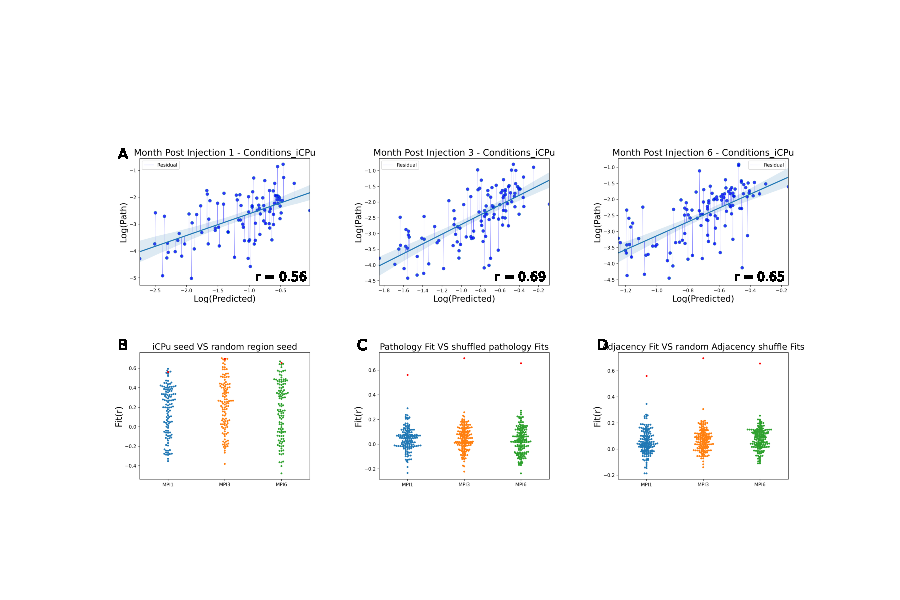
\includegraphics[width=\linewidth]{Figures/Fig2.pdf}
   
    \caption{
      \textbf{Differential regional vulnerability is correlated with $\alpha$-synuclein expression}.
        (\textbf{A}) Conceptual framework for the assessment of regional vulnerability of brain regions. We here show the scatterplot of $\log_{10}$(Predicted) and  $\log_{10}$(Measured) at 6 months post-injection. The black dashed line is the linear regression between prediction and experimental observation. The red area indicates brain regions with higher measured p-$\alpha$-syn staining than predicted by the model, hence 'vulnerable'. Conversely, the green area indicates brain regions with lower observed p-$\alpha$-syn staining than predicted by connectivity, hence 'resilient' brain regions.
        (\textbf{B}) Example of a lollipop plot for the 6 months timepoint highlighting the distance to the mean linear regression (i.e. residues - dashed blue lines).
        (\textbf{C}) Distribution of linear regression residues. The solid blue line is the kernel density estimation of the distribution. 
        (\textbf{D}) Heatmap of the residuals between the predicted and measured p-$\alpha$-syn staining plotted on an anatomical mouse brain as a measure of the relative vulnerability of regions averaged over the 3 experimental timepoints, using the  \textit{Brainrender} package \cite{Claudi_2021}.
        (\textbf{E}) Heat map of the $\alpha$-synuclein mean expression energy values obtained from the Allen Brain Atlas \textit{in situ} hybridization study for each of the designated region. Expression was normalized using min/max to ease visualization. \textbf{Note}: Henderson et al. used a divergent colormap to represent a continous value, hence making it difficult to interpret regional variations. We here chose a sequential continuous colormap to improve the understanding.
        (\textbf{F-H}) Scatterplots of $\log_{10}$(predicted) p-$\alpha$-syn versus experimentally-measured $\log_{10}$(p-$\alpha$-syn) values at 1 month (\textbf{F}), 3 months (\textbf{G}), and 6 months (\textbf{H}). The blue lines are the linear correlations between experimental and predicted values (shaded areas: 95\% confidence interval). Values at the bottom right of each panel are the Pearson's correlation coefficient $r$ between experimental and predicted pathologies. Path: experimentally-measured p-$\alpha$-syn surface.}

\end{figure}

\\
To determine whether model performance could be improved by the addition of other components, Henderson et al. seek out for factors that could contribute to regional vulnerability. An immediate assumption is that local levels of messenger-RNA (mRNA) encoding for $\alpha$-synuclein could influence the future accumulation of $\alpha$-synuclein in aggregates. To directly test that hypothesis, the model was modified to account for regional levels of $\alpha$-synuclein mRNA (\textbf{Figure 2E}) by direclty modifying the adjacency matrix $A = S \times A$, where $S$ is the diagonal matrix of the vector $R$ containing the regional levels of $\alpha$-synuclein mRNA for each brain region of $A$ such as: 

\begin{equation}
  \begin{center}
    $S = $
    \begin{cases}
        $R_{i}$ & \text{for $i = j$} \\
        $0$ & \text{otherwise} \\
    \end{cases}
   \end{center}
\end{equation}
  

Model fitting and performance estimation remained similar. Incorporation of $\alpha$-synuclein trancript's levels in the network diffusion model improved model performance by up 12\% of added explained variance (\textbf{Figure 2F-H}). Here also, we perfectly replicated the original results both qualitatively (shown in \textbf{Figure 2F-H}) and quantitatively (shown in \textbf{Table 3}). Overall, these data suggest that \textit{SNCA} gene expression is an important factor impacting the vulnerability of regions and subsequently pathology spread. 

\begin{table}[ht]
  \begin{center}
    \centering
   
    \begin{tabular}{|l|c|c|} % <-- Alignments: 1st column left, 2nd middle and 3rd middle, with vertical lines in between
      \hline
      
      &\textbf{Henderson et al.} & \textbf{Replication} \hspace{1cm}\\

      \hline
      Best $c$ & $0.414$ & $0.414$ \\
      MPI 1 & &\\
            \hspace{1cm} Pearson's $r$ & $0.580$ & $0.580$\\
            \hspace{1cm} $p$-value & $1.401e^{-9}$ & $1.401e^{-9}$ \\ 

      MPI 3 & &\\
            \hspace{1cm} Pearson's $r$ & $0.727$ & $0.727$ \\
            \hspace{1cm} $p$-value & $2.421e^{-19}$ & $2.421e^{-19}$   \\
            
      MPI6& &\\
            \hspace{1cm} Peasron's $r$ & $0.739$ & $0.739$ \\
            \hspace{1cm} $p$-value & $2.965e^{-20}$ & $2.965e^{-20}$  \\
      \hline
    \end{tabular}
    
    \caption{\textbf{Data correspondence between the original article and the reproduced results using the model incorporating $\alpha$-synuclein mRNA levels.} The results have been rounded up to the third decimal. $P$-values for Pearsonʼs correlation tests were corrected for multiple comparisons using Bonferroniʼs method. MPI: month(s) post injection.}
  \end{center}
\end{table}


\subsection{\textit{In silico} seeding of alternative regions}
To examine the generalizability of the model (\textit{i.e.} the ability to apply to other conditions), Henderson et al. proceeded to \textit{in silico} seeding of alternative regions such as the Piriform Cortex (Pir) and the \textit{Substantia Nigra} (SN). \textbf{Figure ~\ref{fig:fig3}} displays the p-$\alpha$-syn spread at 1, 3 and 6 month(s) post-injection after seeding the model with either the Pir or the SN. We successfully obtained similar predictions after seeding in either the Pir or the SN. \textit{In silico} injection in the Pir remarkably corresponds to previous semi-quantitative p-$\alpha$-syn grading study \cite{Rey_2016} (\textbf{Figure 3A}). On the other hand, \textit{in silico} injection in the SN resulted in slow propagation through the nigrostrial tract to first the caudoputamen and then to cortical regions (\textbf{Figure 3B}). The observed pattern following SN injection mimicks previous experimental results and the staging of human cases \cite{Braak_2003, Recasens_2014,  Bourdenx_2020}. Taken together, these findings support the ability of the Diffusion Network model to generalize data predictions.

\begin{figure}[!h]
    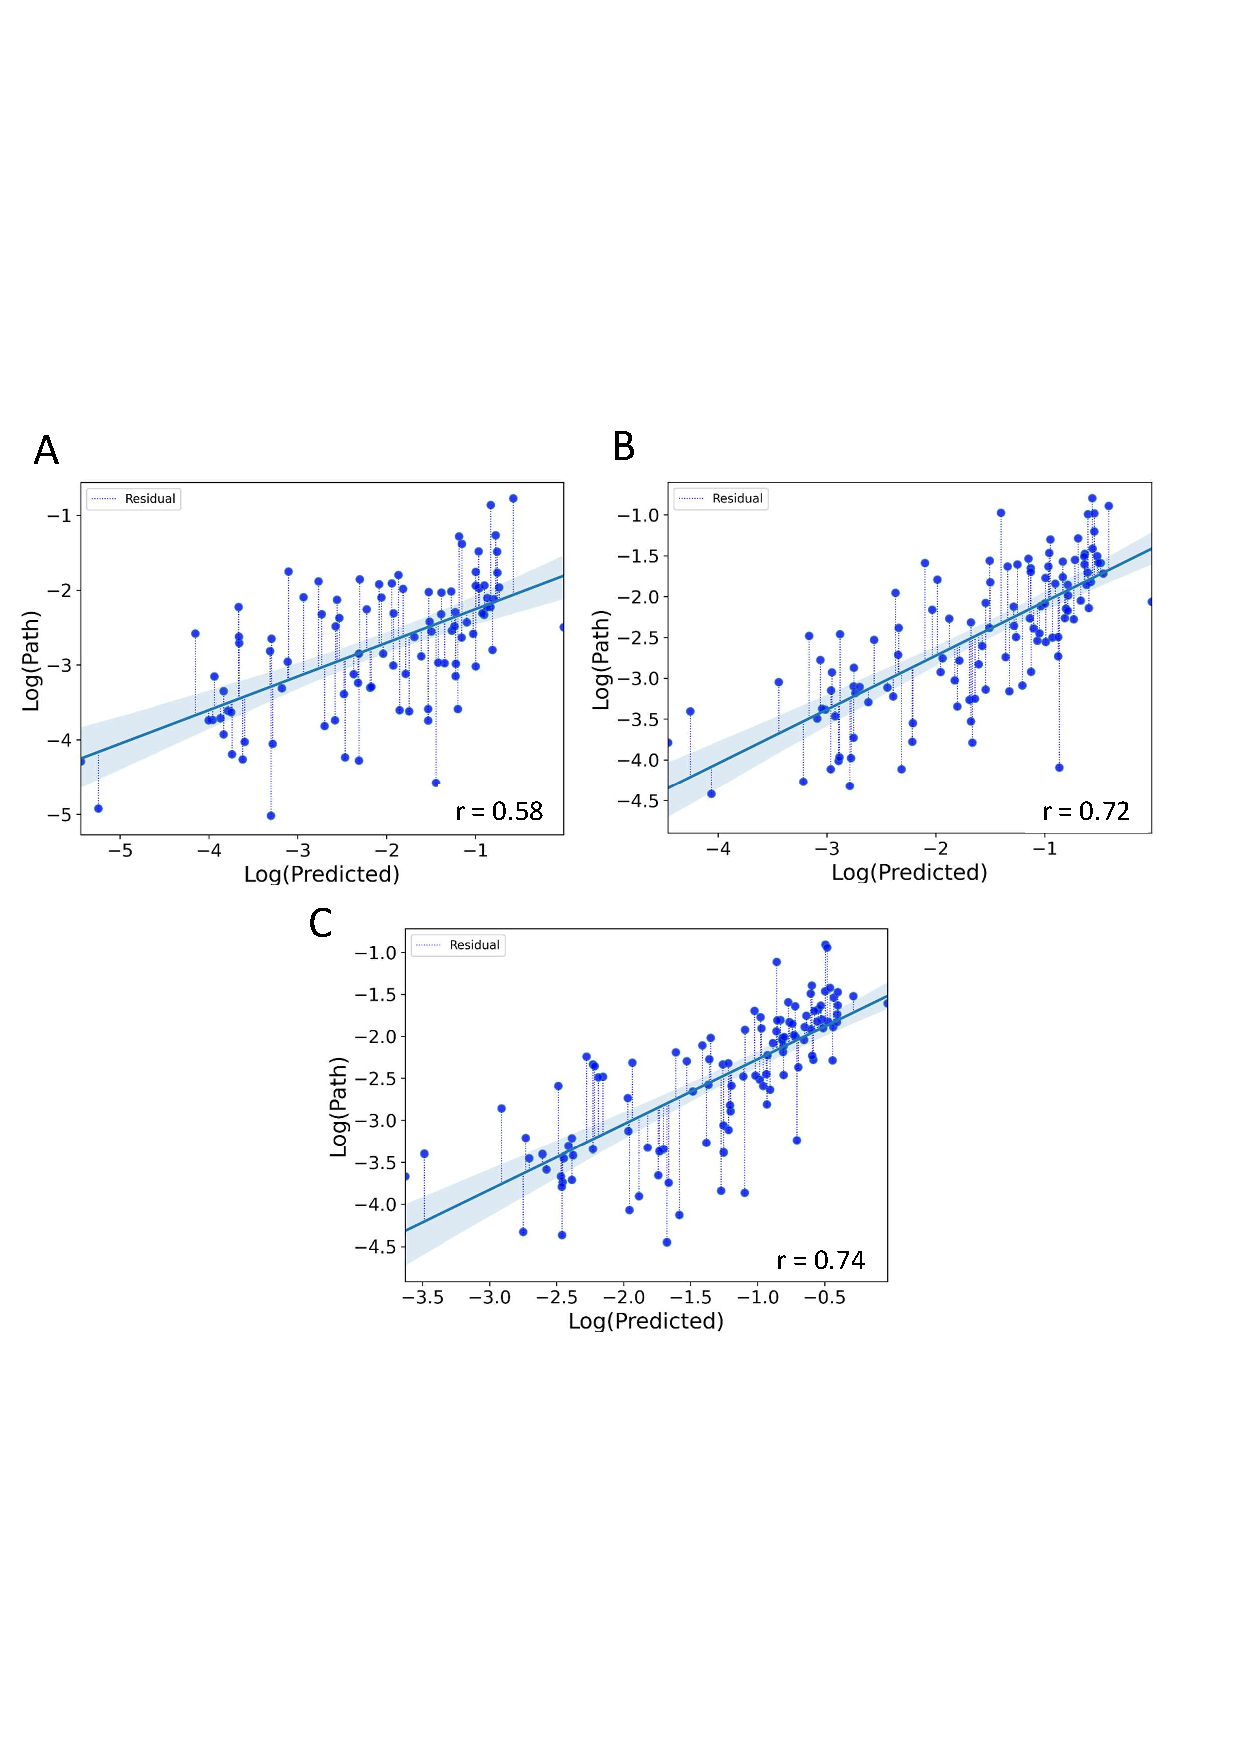
\includegraphics[width=\linewidth]{Figures/Fig3.pdf}

    \caption{\textbf{\textit{In silico} seeding of alternative regions in the mouse brain} 
    Predicted p-$\alpha$-syn staining after \textit{in silico} seeding in the Piriform Cortex (\textbf{A}) or the Substantia Nigra (\textbf{B}) The injection site is indicated on each slice by a blue asterisk. Both Figure A and B are displayed using the \textit{Brainrender} package \cite{Claudi_2021}.}
    \label{fig:fig3}
\end{figure}
    
\section{Conclusion}

In this article, we successfully replicated the computational model created by Henderson et al. \cite{Henderson_2019} in Python.\\
\\
The Network Diffusion Model initially developed by Raj et al. \cite{Raj_2012} and recently adapted by Henderson et al. \cite{Henderson_2019} is a powerful tool to understand the spread of p-$\alpha$-syn in the brain. In its initial form, the model is solely based on anatomical connectivity between brain regions. Despite its simplicity, the model is able to predict 31\% to 47\% of the total variance. In a second version, the endogenous $\alpha$-synuclein expression (at the mRNA level) is added to the model. The addition improves model performance (up to 12\% of added explained variance), although a quantitative analysis should be performed in the future. \\ 
\\
Similarly to what is observed in preclinical models of synucleinopathies or in the brain of Parkinson's disease's patients, $\alpha$-synuclein pathology is composed of 'islands' of vulnerable neurons susceptible to developing pathogenic protein inclusions. By comparing the observed and predicted p-$\alpha$-syn staining based on anatomical connectivity, the model allows to explore regional vulnerability. Finally, seeding in different regions such as the Pir and the SN supports the network diffusion model generalizability. Overall, this model is attractive as it is simple, easily handled, and replicable.\\
\\
Nonetheless, the model is not without limitations. Other experimental datasets (investigating other seeding regions or using alternative markers for pathological $\alpha$-synuclein) are still required to quantitatively assess the ability of the model to generalize the prediction of $\alpha$-synuclein spread. Another barrier comes from the available connectivity data \cite{Oh_2014}. The connectivity matrix used by Henderson et al. and ourselves is at the mesoscale. One implication, for example, is that brain structures are considered homogenous, hence not taking into account the laminar cortical organization for example. The observation of a distinct distribution of the $\alpha$-synuclein pathology in cortical layer suggests that lower scale connectivity data could help to capture overlooked events.\\
\\
Modeling disease propagation in the brain is challenging and often reductionist \textit{per se}. Indeed, during the course of disease, the brain changes according to at least two parallel processes: the "Dynamics \textbf{On} Network" and the "Dynamics \textbf{Of} Network" \cite{Raj_2018}. The first one is related to processes that occur atop a static structure as, for instance, $\alpha$-synuclein spread. The second defines the brain network changes over time (e.g. neurodegeneration or extracellular remodelling \cite{Soria_2020}). A major challenge remains in modeling both these "on" and "of" dynamics. If we were only to understand one dynamic and leave the other dynamic unexplored, we could imagine to still be a step away from the reality of the pathology. 

\section{Acknowledgements}
We thank Dr. Erwan Bezard and Dr. Benjamin Dehay for helpful discussion. T.E.P. was supported by a fellowship from the Encephalia association and M.B. by an 'Allocation Jeune Chercheur' from the Fondation Alzheimer.
